\documentclass[licencjacka]{pracamgr}

\usepackage[english]{babel}
\usepackage{polski}
\usepackage{listings}
\usepackage{color}
\usepackage{url}
\usepackage{pgfplots}
\usepackage{array}
\usepackage{float}
\usepackage{placeins}

\usepackage{amssymb,amsmath,amsthm,amstext,amsopn,latexsym}

\definecolor{mygreen}{rgb}{0,0.6,0}
\definecolor{mygray}{rgb}{0.5,0.5,0.5}
\definecolor{mymauve}{rgb}{0.58,0,0.82}

\newcommand{\code}[1]{\begin{ttfamily}#1\end{ttfamily}}
\newcommand{\Oh}{\ensuremath{\mathcal{O}}}

\newcolumntype{H}{>{\setbox0=\hbox\bgroup}c<{\egroup}@{}}

\lstset{
  backgroundcolor=\color{white},   % choose the background color; you must add \usepackage{color} or \usepackage{xcolor}
  basicstyle=\footnotesize\ttfamily,        % the size of the fonts that are used for the code
  breakatwhitespace=false,         % sets if automatic breaks should only happen at whitespace
  breaklines=true,                 % sets automatic line breaking
  captionpos=b,                    % sets the caption-position to bottom
  commentstyle=\color{mygreen},    % comment style
  escapeinside={\%*}{*)},          % if you want to add LaTeX within your code
  extendedchars=true,              % lets you use non-ASCII characters; for 8-bits encodings only, does not work with UTF-8
  frame=single,                    % adds a frame around the code
  keywordstyle=\color{blue},       % keyword style
  language=C,                 % the language of the code
  numbers=left,                    % where to put the line-numbers; possible values are (none, left, right)
  numbersep=5pt,                   % how far the line-numbers are from the code
  numberstyle=\tiny\color{mygray}, % the style that is used for the line-numbers
  rulecolor=\color{black},         % if not set, the frame-color may be changed on line-breaks within not-black text (e.g. comments (green here))
  showspaces=false,                % show spaces everywhere adding particular underscores; it overrides 'showstringspaces'
  showstringspaces=false,          % underline spaces within strings only
  showtabs=false,                  % show tabs within strings adding particular underscores
  stringstyle=\color{mymauve},     % string literal style
  tabsize=2,                       % sets default tabsize to 2 spaces
  title=\lstname                   % show the filename of files included with \lstinputlisting; also try caption instead of title
}

%Jesli uzywasz kodowania polskich znakow ISO-8859-2 nastepna linia powinna byc 
%odkomentowana
%\usepackage[latin2]{inputenc}
%Jesli uzywasz kodowania polskich znakow CP-1250 to ta linia powinna byc 
%odkomentowana
%\usepackage[cp1250]{inputenc}
\usepackage[utf8]{inputenc}

% Dane magistranta:

\author{Piotr Jaszkowski, Mateusz Machalica, Grzegorz Prusak, Łukasz Solak}

\nralbumu{306249, 305678, 306538, 306462}

\title{Practical Approximation Algorithms Library}
\tytulang{Practical Approximation Algorithms Library}
% Lukasz: potrzebujemy tego?
%\tytulang{An implementation of a difference blabalizer based on the theory 
%  of $\sigma$ -- $\rho$ phetors}

%kierunek: Matematyka, Informatyka, ...
\kierunek{Informatyka}

% informatyka - nie okreslamy zakresu (opcja zakomentowana)
% matematyka - zakres moze pozostac nieokreslony,
% a jesli ma byc okreslony dla pracy mgr,
% to przyjmuje jedna z wartosci:
% {metod matematycznych w finansach}
% {metod matematycznych w ubezpieczeniach}
% {matematyki stosowanej}
% {nauczania matematyki}
% Dla pracy licencjackiej mamy natomiast
% mozliwosc wpisania takiej wartosci zakresu:
% {Jednoczesnych Studiow Ekonomiczno--Matematycznych}

% \zakres{Tu wpisac, jesli trzeba, jedna z opcji podanych wyzej}

% Praca wykonana pod kierunkiem:
% (podaæ tytu³/stopieñ imiê i nazwisko opiekuna
% Instytut
% ew. Wydzia³ ew. Uczelnia (je¿eli nie MIM UW))
\opiekun{Krzysztof Ciebiera\\
  Instytut Informatyki\\
  }

% miesi¹c i~rok:
\date{June 2013}

%Podaæ dziedzinê wg klasyfikacji Socrates-Erasmus:
\dziedzina{
%11.0 Matematyka, Informatyka:\\ 
%11.1 Matematyka\\ 
%11.2 Statystyka\\ 
11.3 Informatyka\\
%11.4 Sztuczna inteligencja\\ 
%11.5 Nauki aktuarialne\\
%11.9 Inne nauki matematyczne i informatyczne
}

%Klasyfikacja tematyczna wedlug AMS (matematyka) lub ACM (informatyka)
% Lukasz: moze cos jeszcze - nie wiem.
\klasyfikacja{
  F. Theory of Computation \\
  F.2. Analysis of Algorithms and Problem Complexity \\
  F.2.2  Nonnumerical Algorithms and Problems \\
}

% S³owa kluczowe:
\keywords{approximation algorithm, C++, monte carlo tree search, local search, steiner forest problem, travelling salesman problem, uncapacitated facility location}

% Tu jest dobre miejsce na Twoje w³asne makra i~œrodowiska:
\newtheorem{defi}{Definicja}[section]

% Macro for problem definitions
\newcommand{\defproblem}[3]{
  \vspace{1mm}
\noindent\fbox{
  \begin{minipage}{0.96\textwidth}
  #1 \\
  {\bf{Input:}} #2  \\
  {\bf{Question:}} #3
  \end{minipage}
  }
}

% koniec definicji

\begin{document}
\maketitle

%tu idzie streszczenie na strone poczatkowa
\begin{abstract}
  We are presenting C++ frameworks for implementing Local Search
  and Monte Carlo Tree Search algorithms. Their design is based
  on 3 NPC use cases: metrical Travelling Salesman Problem,
  Steiner Forest Problem and Uncapacitated Facility Location Problem.
  All design decisions are thoroughly justified. The resulting
  algorithms written in our framework are being compared with
  well known approximation algorithms as described by Vazirani \cite{Vazirani}.
  Our implementations of these algorithms are also provided with the framework.
\end{abstract}

\tableofcontents
%\listoffigures
%\listoftables

\section{Preliminaries}
In this paper, the terms listed below should be interpreted in the following way:
\begin{itemize}
\item Concept\footnote{\url{http://www.open-std.org/jtc1/sc22/wg21/docs/papers/2005/n1758.pdf}}
	-- an interface, which can be required from template arguments.
	On the contrary to polymorphic interfaces, usage of interface elements is resolved at compilation time.
\item Design Pattern\footnote{\url{http://en.wikipedia.org/wiki/Software_design_pattern}}
	-- in our case, it is a weaker requirement than a concept: design pattern has no interface,
	it is just a general guide about responsibilities and expected behaviour of the class
	fulfilling it.
\end{itemize}

\chapter{Local Search Framework design}

\section{Motivation}

Local search\footnote{\url{http://en.wikipedia.org/wiki/Local_search_(optimization)}} is a metaheuristic for solving optimization problems.
It is especially useful when the fitness function's local optima have value close to the global one.
Once a decent topology on the solution space is defined, the algorithm itself is very easy to implement:
you just make a walk in the solution space, choosing every step so that the next solution you "stand in" has
a better fitness than the previous one. The local search implementation has usually just a few dozens of lines and
yet it can generate a series of problem, which usually stay unnoticed:
\begin{itemize}
\item it is hard to test a local search; local searches are prone to bugs:
	\begin{itemize}
	\item correct implementation does not guarantee that the result will be optimal
	\item there is usually no objectively good benchmark instances for problems to which local search is applied
	\item quality of the solution usually strongly depends on the amount of available computational power
	\item nobody bothers to write a decent testing framework (since every local search implementation is different).
		As a result tests are runned by hand, which makes testing prone to human errors (we can easily lose repetitiveness of the results).
	\end{itemize}
\item some parts of code are rewritten in every implementations:
	\begin{itemize}
	\item execution time control
	\item main local search loop
	\item fitness monitoring
	\item step decision making strategy
	\end{itemize}
	Every single of them takes not much code which is hard to generalize anyway.
	However, it is easy to make a bug in these places, which can stay unnoticed for a long time.
\end{itemize}

We've made an attempt to implement a C++ local search 
framework addressing these issues.

\section{General description}

Local Search Framework is supposed to automatize the process of writing local searches with no execution overhead due to the framework code.
Framework should be responsible for making consistent decisions about the issues that are not influencing the algorithm itself
(for example results logging, repetitive testing, limiting execution time) and allow to avoid rewriting repetitive code.
As the concept of local searches is really simple, our design has to be easily comprehensible and super intuitive.
It definitely shouldn't force user to bend/hack the solution to fit the framework.

We use templates and concepts to avoid any overhead in the execution time and allow maximum flexibility.

\section{Main function}

Outer interface of the framework consists of a single template function search().
Its code is explicitly stated in the design - user HAS TO KNOW this piece of code before using the framework.
The order of actions performed is vital for utilization of the framework.
Therefore search() has to be simple and readable for an average user.

We assumed that fitness of the solution can be efficiently calculated and represented as a floating point number.
We believe that imposing the fitness type across the framework is a useful simplification and prevents any type
conversion problems in this context. In the current version fitness type is set to double which is disputable but convenient.

search() doesn't know the nature of the problem.
It is due to the fact that we wanted to extract problem independent components.

Note that search() receives a logger fulfilling the Logger concept defined in the Algorithm
results' presentation framework.


\begin{lstlisting}
template<typename Walker, typename StepCtrl, typename ProgressCtrl,
	typename Random, typename Logger>
void search(Walker &walker, StepCtrl &step_ctrl, ProgressCtrl &progress_ctrl,
	Random &random, Logger &logger)
{
	while(1)
	{
		double current_fitness = walker.current_fitness();
		logger.log(current_fitness);
		double progress = progress_ctrl.progress(current_fitness);
		if(progress>=1) break;
		walker.prepare_step(progress,random);
		if(step_ctrl.step_decision(current_fitness,walker.next_fitness(),
			progress,random)) walker.make_step();
	}
}
\end{lstlisting}

\section{Concepts}

\subsection{Walker}

Walker is the only component which knows the nature of the problem.
It is not divided on this framework level, since if more components would know about the problem it would create cross dependencies.
In other words, such situation would inevitably make search() to transfer problem specific data between them.
Also many custom/intrusive optimization can be made at this point, so we believe that this is definitely a point at which we should allow user to plug in
his own code.

Walker is responsible for:
\begin{itemize}
\item maintaining the current solution
\item preparing the proposition of the new step
\item making the proposed step
\end{itemize}

It has to contain an initial solution before calling search().
Better solutions have lower fitness.

\subsection{ProgressCtrl}

ProgressCtrl (Progress Controller) controls the execution time of the
local search. It is responsible for estimation of the ratio: iterations
passed/iterations available.

It is usually implemented as a time/iteration limit or solution sufficiency threshold.
None of these are problem dependent, hence this component can be effectively extracted from the design.

\subsection{StepCtrl}

StepCtrl (step controller) represents the metaheuristic chosen to
solve the problem. It is responsible for making decision whether to
make the step proposed by Walker.
Simulated annealing and hill climb have easy/trivial implementations of this concept.

\subsection{Random}

It is just c++11 RNG concept.
Random (Pseudo Random Number Generator) generates random integer values.
It is explicitly shared between components of the search() for the following reasons:
\begin{itemize}
\item we assume that we receive only one seed from the outside
\item using many generators at once (especially with the same seed) may create undesired conditional probabilities
\end{itemize}

\section{Reasoning}

We have considered approaches alternative to the proposed design, they are
worth studying in order to identify possible problems and why current design
solves them in our opinion.

\subsection{Abstract representation}
It is helpful to express structure of local search framework in terms of a
graph where each node represents a separated concept and an edge $A \to B$
exists iff concept $A$ uses (e.g. calls, owns, reads data) concept $B$. First
assumption was that resulting graph is compact, local search algorithm provided
by the framework should be seen as one phase from the outside (e.g. invocation
of one function, which takes input and returns result), so every concept in
different connected component than the algorithm itself is useless. We will
refer to described graph as the \emph{component graph}.

\subsection{The way to the tree}
We have eliminated all designs with cycles in component graph, the most
important reason for this was that we could not find how we can benefit from
allowing two way communication between components. Furthermore all concepts
need to be initialized either by user or search procedure itself if they are
completely algorithm independent (like statistics gathering) and every cycle
makes initialization really complicated, there is no arbitrary choice of
initialization order we could come up with in this case.

Therefore we were free to choose either general DAG or a tree (we were aiming
for the latter). To reduce both of them to the second one we can run
depth-first search from algorithm's entry point (the search() procedure), which
becomes a root of a depth-first spanning tree. The only difference between the
graph being a general DAG and a tree is manifested by the presence of non-tree
edges. Our graph is acyclic, so we will not find back edges.

Please note that presence of back edges would mean that execution flow can be
returned to caller for a moment and then returned back to the callee
automatically - this can obviously be replaced by making communication
passive, caller provides all data needed do execute call (query) and expects
response, every query is initiated by caller and completed by callee using
provided data.

\subsection{Forward edges elimination}
Any forward edge means that we are skipping many abstraction layers with an
invocation. Obviously this can be avoided by passing a call through all layers
that are bypassed by a forward edge. We replace forward edge with composition
of facades. Modern C++ compilers can easily inline such constructions, so that
the forward edge will not be present in design and C++ code, but will be
generated by compiler for performance reasons.

Moreover every forward edge means that at least two different concepts need to
know (the same) type of called concept, we think it is less convenient during
initialization, however in this specific case a concept can inherit type from
its predecessor in the spanning tree (as long as the former is not initialized
by a user).

We have made an experiment with changing parts of an algorithm (namely
underlying data structure) during algorithm execution. Obviously allowing
forward edge in this case (calling specific data structure directly, skipping
its owner) might invalidate algorithm. The real problem here is a stupid user
who gave an ownership to the object being descendant of a caller while allowing
forward edges in the component graph. Removing forward edge as described above
forces every call to pass through data structure owner, which is less
error-prone and simpler.

We further assume that there is no forward edges in the graph.

\subsection{Cross edges discussion}
Consider the case where one concept $C$ is a child of two (or more) concepts
$A$ and $B$ (assume $B \to C$ is a cross edge). Let $P$ be the lowest common
ancestor of both $A$ and $B$ in depth-first spanning tree of the component
graph. Described situation breaks composability of algorithm's design but one
can easily come up with an example of a local search algorithm where such
design is desired, we will discuss it later, for now let us assume that we do
need communication between components as described above.

If we disallow cross edges in our design we have to provide different mechanism
of communication between $B$ and $C$. As the graph without cross edges is a
tree we have to pass data back (query result) from $C$ to $P$ and provide $B$
with it in separate call. The obvious problem here is that data format must be
know to all concepts on paths from $B$ and $C$ do $P$ (including $P$) and data
format type can (in most cases will) be domain dependant - therefore we are
raising domain boundary up to lowest common ancestor of components that were
connected by cross edge. This means that protocol common to $B$ and $C$ (which
may change) must be propagated during initialization down in the tree starting
from $P$.

The obvious benefits from tree-like component graph is simple. In top-down
initialization, we can assume that during construction of algorithm child being
initialized is given an interface to obtain initialization data from parent
according to its needs or this data is passed explicitly. Furthermore there is
no problem with assigning an ownership of a concept. Tree design makes
synchronization model extremely easy to implement in case one would like
concepts to operate concurrently.

There are more problems with cross edges. Initialization cannot be done
top-down in described automatic fashion, ownership assignment just like the
rest of the initialization procedure needs to be done by the user as hidden
dependencies are not obvious to any automatic model. It is pretty obvious that
the less constraints we put on algorithm's design the less we know and the more
must be done manually.

It turned out that in the case of local search framework both performance
considerations and domain-dependency limiting required nearly the same
transformations of components graph, which resulted in the graph becoming a
tree. Cross edges were eliminated by encoding entire problem specific
components in the Walker concept. Topologies of solution spaces implied by
problems discussed when designing this framework vary considerably, we were
unable to split this concept leaving complexity of single step unchanged for
studied examples.

\section{Framework supplied implementations}

\subsection{ProgressCtrl implementations}
\begin{itemize}
\item IterationCtrl - fixes the number of search iterations.
\item TimeCtrl - fixes time of search execution up to to the fixed granularity.
	Granularity is the amount of iterations between the consecutive time checks.
	Checking time every iteration is too expensive if expected single iteration time
	is very short.
\item TimeAutoCtrl - same as TimeCtrl but the granularity is being adjusted
	automatically using linear regression. The aimed gap between time checks has
	been hardcoded to $0.01s$.
\end{itemize}

\subsection{StepCtrl implementations}
\begin{itemize}
\item HillClimb - accepts a step if the next fitness is better than the current fitness.
\item Annealing - makes a decision according to the temperature schedule defined by
	Boltzmann distribution\footnote{\url{http://en.wikipedia.org/wiki/Boltzmann_distribution}}
\end{itemize}

\subsection{Walker implementations}
Particular walkers are described in the chapters about the problems they operate on.
\begin{itemize}
\item TSP: TwoOptWalker
\item UFL: BestStepWalker, RandomStepWalker
\item Steiner Forest: [TODO]
\end{itemize}


\chapter{Monte Carlo Tree Search framework design}

\section{Preliminaries}
Describing optimisation problem in terms of finding a sequence of decisions
that result in optimal solution seems natural to humans. In the this chapter we
will describe related approach used widely in combinatorial optimisation and
artificial intelligence. We assume reader to be familiar with the concept of
\emph{decision tree}
\footnote{\url{http://en.wikipedia.org/wiki/Decision_tree}}.

\section{Motivation}
\emph{Monte Carlo Tree Search} (MCTS) is a metaheuristic for finding
near-optimal decisions in the decision space by building the search tree and
evaluating its nodes according to random simulations.
MCTS is an iterative method, samples from many iterations are combined together
so that the best (or rather the most promising) decision from the current state
can be chosen based on aggregated statistics.

To implement MCTS-based approximation for given problem two domain-specific
components must be defined: an evaluation function which gives a linear ordering
of feasible solutions and an algorithm for enumerating all possible states
reachable from given one by making a single decision.
Both of these parts are usually simple, but MCTS algorithm itself is not. Many
problems may be encountered when implementing the algorithm:
\begin{itemize}
  \item maintaining and traversing tree structure requires plenty of tedious
    and error prone code, memory utilisation is a significant problem given the
    number of simulations that can be performed using modern computers
  \item statistics gathering and utilisation code cannot be tested in any reasonable way
    \begin{enumerate}
      \item correct implementation is, in most cases, not guaranteed to find the optimal solution
      \item errors can cause slight regression or improvement depending on test instances
      \item numerical stability of statistics manipulation procedures is a
      problem that a few would expect from combinatorial optimisation algorithm
    \end{enumerate}
  \item there is a number of components that are common or interchangeable
    amongst the majority of MCTS method implementations, each of these parts is
    worth generalisation due to virtually no coupling with approximated problem
    \begin{itemize}
      \item tree structure modifications and traversing
      \item time execution control
      \item statistics aggregation and optimal decision extraction
      \item efficient decision and state propagation
    \end{itemize}
\end{itemize}

Proposed framework is our attempt to address these issues.

\section{General description}
Nomenclature introduced in this section is similar to the one used in
\cite{MCTSsurvey}.  Let us recall the basic operation of MCTS algorithm, for
more precise description please refer to mentioned publication.

MCTS method finds single near-optimal decisions from the current state (which
will be sometimes called \emph{root state}) according to statistical
information gathered from a number of iterations. A single iteration can be
divided into three phases.
We start by choosing the most urgent node of a tree using \emph{tree policy}.
We will usually think about this process as making a walk from the root of a
tree to some node. Choosing appropriate tree policy allows us to maintain
balance between exploration and exploitation.
As a result of applying tree policy we may reach a leaf of the tree,
representing state which is not necessarily terminal, as we don't want to store
entire tree in the memory. It is tree policy's responsibility to decide whether
to expand this leaf by creating a new child node for each state which can be
reached with a single decision.
Starting from this node (state) we use \emph{default policy} to evaluate it, in
the simplest case default policy will make a random sequence of moves until
terminal state (which can be evaluated directly) is reached.
The result of an evaluation is propagated backwards (up to the root) and statistics
in each node are updated.

Note that after performing the desired number of simulations one can choose the
most promising (according to aggregated statistics) decision and update the
current state. In order to find near-optimal solution one usually needs to find
a sequence of decisions that lead from arbitrary state to some terminal state
representing feasible solution. This is obviously trivial if one has an
algorithm that finds a single decision. We will discuss possible methods of
performing this task later in this chapter.

\section{Search tree format}
One can choose from two opposite approaches to represent a search tree.

One approach is to identify each node of a tree with concrete state and connect
them with edges (identified with decisions) in such a way that children of a
given node are those states that can be obtained from the parent node's state by
making a single decision. It should be obvious that initial state -- the one from
which we want to make a decision at the moment -- is represented by the root of
the tree.

The other approach would be to store initial state in the root, but instead of
storing states one can store transitions between them -- possible decisions.

Both ways may seem identical conceptually, but they are quite different from
the algorithmic and technical points of view.
Imagine a problem where updating state after making a single decision is an
expensive process, in such case the states-oriented implementation can improve
performance of simulation -- we would save the cost of applying decision to the
states placed near root node in the search tree.
On the other hand computer a representation of an entire state tends to be much
larger than representation of a single decision, in such situations second
approach can save us both time and memory.
We could not come up with reasonable problem and solving strategy based on
MCTS, where the first approach has any advantages over the second one. Therefore we
provide a framework for building algorithms using the second approach only.

There is a one (quite ugly) hack that can be done in order to implement search
tree structure similar to the first approach using our framework. Since state
description, decision representation and aggregating function that applies
decision to given state and produces new one are specified by user one can do
things as follows: state would stay unchanged, decision will be described not
by an incremental but as a full destination state and aggregation function
should discard source state and return destination one encoded in 'decision'.
If properly implemented by a user this can be used with our framework with
virtually no overhead. Therefore the chosen approach is at least as expressive
(when memory and complexity constraints are taken into account) as each of
proposed.

\section{Domain dependency}
Our goal was to limit a coupling between specific problem and our framework, we
have decided to restrict domain-specific part of a MCTS-based algorithm to two
components, namely State and Move. Referring to previously introduced
nomenclature, States coincide with abstract states (nodes in the tree) and
Moves -- with decisions (edges in the tree).
The Fitness is a separate concept describing the result of and an evaluation of a
state. We have assumed that Fitness is represented by a linearly ordered set
which is isomorphic with a subset of double type. Except for theoretical
precision issues, we found no drawbacks of this simplifying decision for any
real life MCTS application.

\section{Concepts}
We have identified a few concrete components of MCTS algorithm, that are in our
opinion generically atomic.

\subsection{Payload}
The Payload concept maintains statistics describing single state, that are used
by the Policy concept. The Policy is also the only component that can access, modify
and understand information enclosed in Payload. Node, being only an owner of
the payload object, indirectly stores the assignment between state and payload.

Tree nodes are part of the tree while aggregated statistics are conceptually
connected with tree policy, we could not store them in the nodes directly.

\subsection{Policy}
The Policy concept coincides with the tree policy described before.
All examples discussed and implemented during the course of designing this
framework reduced the problem of finding the most urgent node in entire tree to
finding locally the most urgent child to descend into and in consequence
finding a path to chosen node from the root. Therefore tree policy provides a
function that given a node, a state reached in this node and its children
returns child that should be examined recursively. An alternative approach would
involve passing the entire tree structure to the decisive function. By requesting
local decisions we make this simple both conceptually and technically yet
described interface has enough expressive power. We have never came up with nor
found in the literature a reasonable strategy that requires global information
about the search tree.
Building path from the root node enables us to limit the effects of performing
a single simulation to a reasonable number of nodes, since after evaluating chosen
node we update all nodes on the path to the root and only them.

Possible domain-dependency of the tree policy is theoretically allowed since
local decision is made based on entire information stored in the node and the
state reached by making decisions encoded in edges traversed during node
selection.
This possibility is usually ignored since it has been proven that MCTS
algorithms are extremely efficient when implemented as metaheuristics, without
any knowledge about the problem other than default policy and some black-box
algorithm to generate states reachable from given one by making a single
decision. In such case tree policy makes a decision based on aggregated results
of previous simulations only.
This is also an approach that we choose for our framework.

Policy is also responsible for propagating consequences of making single
sample in the tree. Its update procedure is issued for each node on the path
from chosen node to the root (in this order).

Once the algorithm reaches the most urgent node it has to decide whether to expand
it -- create child nodes for each state reachable by making a single decision.
The Policy concept provides a predicate which answers this question based on
reached node and its level in the tree (number of nodes on the path to tree's
root).

\subsection{Move}
Move is an increment representing a single decision. It is stored in the search
tree instead of full state and incrementally applied to the state when making
simulations. Has no important role and is completely dependent on the State.

\subsection{State}
State is a main component that encodes specific problem in MCTS algorithm.  It
is responsible for full implementation of the default policy, evaluation of Fitness
for a given state, generating Moves that can be done from current state and
establishing connection between Move and itself.

Note that from the framework's point of view there is no assumption about how
default policy estimates state's Fitness, there is no need for the state to
apply a random sequence of moves to itself in order to obtain terminal state
which can be evaluated directly, this technique is pretty common though (and
advised as a good starting point).

It is beneficial to walk through the process of choosing node by the Tree
(according to Policy component). We start at the root by copying initial state
and then we feed the copy with Moves found on the edges traversed according to
the decisions of the tree policy, therefore each time we need to provide some
component with the state of current node we can answer this request without
storing state in each node. This also means that State must provide a procedure
to modify itself based on provided Move.

\section{Possible modifications}
In every experimental implementation we have created to test our design, we
have observed that each component is monolithic. Splitting (always possible,
not always desirable) would make things slower and harder to implement or
understand.

The question is whether it is possible to merge some of presented components.
Since MCTS algorithms are widely used in games application we had some
intuition where to draw the line between domain dependent and independent
parts. The design is very flexible and as it was said one can move this
boundary making virtually everything domain-aware. It is obvious that State
and Move components must be separated even thought they are strongly connected
with each other, this separation must be visible from the Tree's point of view
for efficiency purposes.
Merging Payload with Tree (actually a node in the tree) would make most of the
code dependent on Policy component or memory inefficient and harder to modify
if node would store some predefined set of statistics.
Policy component is critical -- it is domain-independent in most cases and
there exist many implementations easily interchangeable between different
problems.

\section{Finding decision sequence}
Our framework covers the problem of finding optimal decision given initial
state. The natural extension to finding a feasible solution (which is hopefully
near-optimal) or equivalently a sequence of decisions, can be done by
iteratively finding and applying decision until terminal state (and therefore a
feasible solution) is reached.

The reason why we decided not to implement the additional loop should be
obvious. The simple loop approach is probably the worst one can come up with.

As the number of decisions made increases the reachable state space shrinks (in
most cases exponentially, otherwise our approximation is as slow as brute-force
algorithm) therefore it sounds reasonable to reduce the number of simulations
per one decision.

For some problems we can approximate the size of the state space reachable from
current state and if it is smaller than some problem and implementation
dependent value it might be profitable to perform an exhaustive search instead
of random sampling. This typically increases accuracy of the approximation and
in some cases reduces the time and space cost as we have no overhead on maintaining
the structure and meta data kept in the search tree. This approach has been proven
to work in many game solving applications of MCTS and introduced an improvement
confirmed by our tests.

\section{Framework supplied implementations}

Together with MCTS framework we provide several implementations of concepts
which are domain independent and interchangeable between problems. Examples
include tree policies widely used in games solving MCTS algorithms.

In all cases expand decision and Fitness estimation are independent one from
another. To avoid writing all possible combinations we created components which
implement one or the other part of Policy's functionality, we put them together
using inheritance.

\subsection{Expansion strategies}

We provide only one strategy which allows expansion of a given node when the
number of visits reaches some user-defined value. For problems where branch
factor of the decision tree is well defined, the expansion threshold should be
set to the mean branch factor of the tree as described in \cite{Pawlewicz}.
Too big values of the expansion threshold lead to small trees and disable add
node selection logic, on the other hand too small values result in a huge tree
which cannot be stored in RAM.

\subsection{Estimation and node selection strategies}

These include (we refer to the node chosen for the next simulation as the most
urgent node and to the node returned after all simulations are performed as the
best node)
\begin{itemize}
  \item \emph{PolicyRandMean} -- choosing node at random when finding the most
    urgent node, the best node is the node with the lowest mean of collected
    estimates
  \item \emph{PolicyEpsMean} -- choosing node at random with probability
    $\epsilon$, otherwise choosing currently the best node as the most urgent
    one, the best node is the one with the lowest mean of collected estimates
  \item \emph{PolicyEpsBest} -- as above but the best node is the one with the
    lowest minimum of collected estimates
  \item \emph{PolicyMuSigma} -- choosing node with the lowest mean + standard
    deviation of collected estimates, this is the best node too
\end{itemize}


\chapter{Algorithms' results presentation design}
\section{Motivation}

The interest of the contemporary researchers in the field of algorithms 
focuses on problems to which no unambiguously good solution is known. As new heuristic algorithms solving the
particular issue are developed, there arises a need of comparison of their
quality. This meta problem is very generic in its nature and hard to handle,
taking into constideration the variety of approaches the specialists are using.
As a result it is usually troublesome to make a reliable statistics among programs
written by different people or even repeat someone else's empirical results. (not to mention
the fact that it is often hard to access the source code a published paper is
based on).

For the purpose of this paper we have developed our own framework
for homogenuous and repetitive transformation of the algorithm output to a
publishable result. Together with a concept capable of wrapping virtually any
type of algorithm, we've obtained a framework which should allow anyone to
repeat experiments written by other people in his own execution environment
and plug in his own solution to make a reliable comparison.

\section{General description}

[design pattern] Table[/Report] - Impersonates any type of visual report.
	It is responsible for running an algorithm (see Algorithm concept), providing
	it with a logger (see Logger concept), processing logs and collecting human
	readable data. It should be prepared to handle some user defined class of
	algorithms. Intuitively, every diagram, table, grid with results, etc. should
	have its own specialized Table. Table is only a design pattern, since is too
	general to enforce any specific interface on it.

[concept] Algorithm - Encapsulates an algorithm execution. It is responsible for
	initialization of the specific algorithm (for example: obtaining seed, 
	selecting problem instance, setting execution constants, selecting strategies,
	etc.), running the algorithm itself, logging statistical data for Table
	(or at least transfering down the logger) and collecting the results.

[concept] Logger - it is supposed to effectively harvest the relevant information
	about the performance basing on the fitness (assumed to be ultimate measure).
	The actual behaviour of the Logger is chosen by Table instance, however
	Logger's interface (consisting only of log() method) is fixed,
	since similarly to PRNG it is propagated downward (i.e. it is intrusive).

\section{Concepts}

\section{Framework supplied implementations}


\chapter{Metrical TSP algorithms}


\section{Problem description}

\defproblem{ Metrical Travelling Salesman Problem}
{ Complete graph $G = (V,d)$, where $d:V \times V \to\mathbb{R}$ is a metric. }
{ What is the shortest cycle in $G$ which comes through every vertex exactly once? }

See link\footnote{\url{http://en.wikipedia.org/wiki/Travelling_salesman_problem}}
for detailed description.

\section{Christofides 1.5-apx}
Christofides algorithm\footnote{\url{http://en.wikipedia.org/wiki/Christofides_algorithm}} is designed to work with instances of TSP whose edge
weights satisfy triangle inequality. Let $G=(V, w)$ be an instance of TSP,
the algorithm consists of four steps:
\begin{enumerate}
\item Create minimum spanning tree $T$ for graph $G$. \\
Here we have implemented $\Oh(n^2)$ Prim's algorithm\footnote{\url{http://en.wikipedia.org/wiki/Prim's_algorithm}}.
Although for Euclidean spaces there exists faster $\Oh(n\log(n))$ algorithm, the overall gain
would be insignificant so we didn't use it.
\item Let $O$ be a set of odd degree vertices in $T$.
	  Find minimum perfect matching $M$ in complete graph over $O$. \\
For this part we have used \textit{Blossom V}\footnote{\url{http://pub.ist.ac.at/~vnk/software.html}}
implementation of Edmond's Blossom algorithm\footnote{\url{http://en.wikipedia.org/wiki/Blossom_algorithm}}.
Worst case running time of this part is $\Oh(|O|^5)$ but in average case it behaves very well.
\item Combine edges of $M$ and $T$ to form a multigraph $H$.
\item Find Eulerian circuit $E$ in $H$. ($\Oh(|H|)$).
\item Make $E$ Hamiltonian by shortcutting visited nodes. ($\Oh(|E|)$).
\end{enumerate}
Summing this up, our implementation in worst case needs $\Oh(|V|^5)$ time but generally
is fast in comparison to our other techniques.

\section{2opt Local Search}

In 2-opt\footnote{\url{http://en.wikipedia.org/wiki/2-opt}} local search for TSP, a single step
consists of reverting a segment of the current cycle. Intuitively, we find a point
at which the route crosses over itself and reorder it so that is doesn't.

Since in metrical TSP distance between a pair of points is the same for both directions,
computing fitness of the new route simplifies to replacing a pair of edges and replacing it with another
pair.

We've tested 3 different structures for maintaining the current local search solution:
\begin{itemize}
\item array of vertices in order as they appear on the cycle.
\item Reversible Segment List\footnote{\url{http://www.hars.us/Papers/revi.pdf}}
\item Augmented splay tree.
\end{itemize}

\begin{tabular}{c|cc}
& vertex read cost & reverse cost \\\hline
array & $\Oh(1)$ & $\Oh(|V|)$ \\
RSL & $\Oh(\sqrt{|V|})$ & $\Oh(\sqrt{|V|})$ amortized \\
splay & $\Oh(\log(|V|)$ amortized & $\Oh(\log(|V|))$ amortized
\end{tabular}

In our implementation segment to reverse is selected with uniform probability,
excluding the degenerated cases - set of cycle edges has to actually change.
Evaluating fitness of neighbouring solution drawn requires to read vertices
on 4 positions in the cycle. The number of fitness evaluations dominates
the number of the actual reverses in the long run due to the fact that it
becomes harder and harder to find a neighbour with better fitness as we approach
the local optimum. As a consequence we have empirically observed that out of
3 data structure mentioned, the array performed best on TSPLIB (see Benchmarks)
test cases.

\section{Monte Carlo Tree Search}
\section{Benchmarks}
To evaluate the algorithms quality we have used TSPLIB\footnote{\url{http://comopt.ifi.uni-heidelberg.de/software/TSPLIB95/}}
symmetrical instances.
\section{Results}



\chapter{Steiner Forest algorithms}

\section{Problem description}
Steiner Forest Problem (SFP)\\
Given an undirected graph $G = (V, E)$, a cost function on edges $c : E \rightarrow Q^+$, and a collection of disjoint subsets of $V$, $S_1, \dots S_k$, find a minimum cost subgraph in which each pair of vertices belonging to the same set $S_i$ is connected.
For $k = 1$ the problem is known as Steiner Tree Problem (STP).

\section{Primal-Dual Method algorithm}
Local searches written in our framework were compared to a 2-approximation algorithm described by Vazirani [Vazirani]. As far as we know, it's the best approximation algorithm for a SFP known to date.

Time complexity of provided implementation is $\Oh(S(E + V\alpha(V) + \log(S)))$ where $S = \sum_{i = 1}^{k}S_i$, $\alpha(V)$ is the inverse of the function $n = f(x) = A(x, x)$ and $A$ is Ackermann function.

\section{Create and break cycle local search}
Given some solution to Steiner Forest Problem ,,Create and break cycle'' (CBC) local search changes it by randomly adding edge between solution's vertices. If added edge created a cycle then the heaviest edge from this cycle is removed. It's obvious that obtained graph is still a feasible solution. After described operation it might happen that some edges are no longer needed like for example edges adjacent to leafs that don't belong to $S_i$ for any $i \in \{1, \dots k\}$. Therefore pruning procedure is used to ensure that only essential edges remains which might lead to further fitness improvement.

Provided Walker implementation takes $\Oh(V\log(V) + KV)$ time to prepare a step, where $K$ is a limit of attempts to choose a random edge with propierties as described above. In practice the limit is hardly ever reached and preparing step takes $\Oh(V\log(V)$.

\section{Minimum spanning tree of active vertices local search}
,,MST of active vertices'' (MSTAV) local search starts with some feasible solution of SFP. At each step a new solution is created by computing a pruned minimum spanning tree of $G'$ which is a subgraph of $G$ induced by some set of vertices $V'$ called active vertices. $V'$ is obtained from vertices belonging to the previous solution after randomly applying one of the following operations:
\begin{itemize}
\item add a random vertex that's not already in the set,
\item remove a random vertex from the set,
\item do both operations described above.
\end{itemize}

Note that it might happen that there is no feasible solution in $G'$. Therefore at the end of each step local search checks whether proposed solution is feasible and if it is not then it reverts any changes.

Provided Walker implementation takes $\Oh(E \log(V))$ time to prepare a step.

\section{Benchmarks}
To compare the algorithms we have used our randomly generated tests and a subset of SteinLib\footnote{\url{http://steinlib.zib.de}} tests for Steiner Tree Problem.
Names of tests generated by us can be expressed as regular expression $[s\ |\ d][E\ |\ R]V<\text{vertices count}>K<\text{terminal vertices count}>$. Letters $s, d$ tells whether graph is sparse or dense and letters $E, R$ tells accordingly whether graph is Euclidean or if edges were given random weight. Descriptions of SteinLib tests can be found at \url{http://steinlib.zib.de}.

In every test Walker starts with a pruned MST as starting solution.
\section{Results}

\subsection{Comparison of hill climbing and simulated annealing convergence}
\FloatBarrier
Experimenting with Walkers utilizing StepCtrl that use hill climb and simulated annealing (SA) strategy we have noticed that simulated annealing does not improve fitness of found solutions.
If we consider how presented local searches change depending on StepCtrl we can gain some insight why this happens.
Note that CBC could benefit from SA strategy only when in consecutive iterations choosen edges would create a path leading to cycle creation. There is a little probability for such event a specially because solution is pruned every time edge creating cycle is found. As for MSTAV it allows for adding vertices that might not improve solution immediately which is exactly what we would expect from simulated annealing strategy.

\begin{figure}[hb]
\pgfsetplotmarksize{0pt}
\begin{figure}
 \centering
 \caption{\label{CBC-02dEV100K30}CBC-02dEV100K30},
 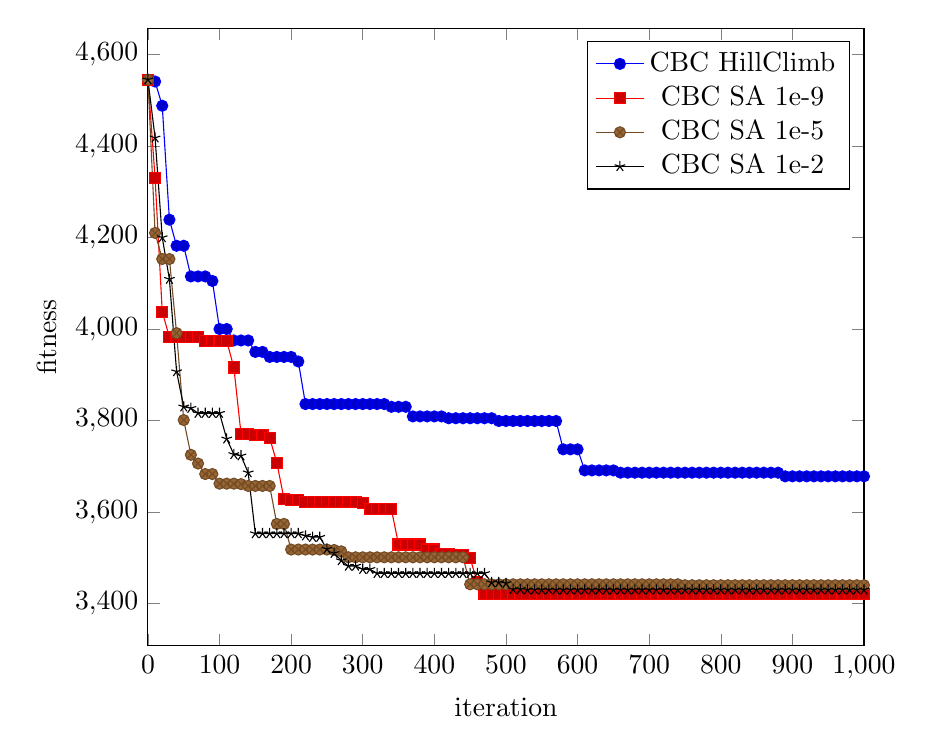
\begin{tikzpicture}
 \begin{axis}[
   width=0.75\textwidth,
   scale only axis,
   xlabel=iteration,
   ylabel=fitness,
   xmin=0,xmax=1000,
   domain=0:1000]
   \addplot coordinates {
     (0,4545)
     (10,4541)
     (20,4488)
     (30,4239)
     (40,4182)
     (50,4182)
     (60,4115)
     (70,4115)
     (80,4115)
     (90,4105)
     (100,4000)
     (110,4000)
     (120,3975)
     (130,3975)
     (140,3975)
     (150,3950)
     (160,3950)
     (170,3939)
     (180,3939)
     (190,3939)
     (200,3939)
     (210,3929)
     (220,3836)
     (230,3836)
     (240,3836)
     (250,3836)
     (260,3836)
     (270,3836)
     (280,3836)
     (290,3836)
     (300,3836)
     (310,3836)
     (320,3836)
     (330,3836)
     (340,3830)
     (350,3830)
     (360,3830)
     (370,3809)
     (380,3809)
     (390,3809)
     (400,3809)
     (410,3809)
     (420,3805)
     (430,3805)
     (440,3805)
     (450,3805)
     (460,3805)
     (470,3805)
     (480,3805)
     (490,3799)
     (500,3799)
     (510,3799)
     (520,3799)
     (530,3799)
     (540,3799)
     (550,3799)
     (560,3799)
     (570,3799)
     (580,3737)
     (590,3737)
     (600,3737)
     (610,3691)
     (620,3691)
     (630,3691)
     (640,3691)
     (650,3691)
     (660,3686)
     (670,3686)
     (680,3686)
     (690,3686)
     (700,3686)
     (710,3686)
     (720,3686)
     (730,3686)
     (740,3686)
     (750,3686)
     (760,3686)
     (770,3686)
     (780,3686)
     (790,3686)
     (800,3686)
     (810,3686)
     (820,3686)
     (830,3686)
     (840,3686)
     (850,3686)
     (860,3686)
     (870,3686)
     (880,3686)
     (890,3678)
     (900,3678)
     (910,3678)
     (920,3678)
     (930,3678)
     (940,3678)
     (950,3678)
     (960,3678)
     (970,3678)
     (980,3678)
     (990,3678)
     (1000,3678)
   };
   \addlegendentry{CBC HillClimb}
   \addplot coordinates {
     (0,4545)
     (10,4330)
     (20,4038)
     (30,3982)
     (40,3982)
     (50,3982)
     (60,3982)
     (70,3982)
     (80,3974)
     (90,3974)
     (100,3974)
     (110,3974)
     (120,3916)
     (130,3771)
     (140,3771)
     (150,3768)
     (160,3768)
     (170,3762)
     (180,3708)
     (190,3629)
     (200,3626)
     (210,3626)
     (220,3621)
     (230,3621)
     (240,3621)
     (250,3621)
     (260,3621)
     (270,3621)
     (280,3621)
     (290,3621)
     (300,3619)
     (310,3606)
     (320,3606)
     (330,3606)
     (340,3606)
     (350,3529)
     (360,3529)
     (370,3529)
     (380,3529)
     (390,3518)
     (400,3518)
     (410,3508)
     (420,3508)
     (430,3506)
     (440,3506)
     (450,3499)
     (460,3446)
     (470,3420)
     (480,3420)
     (490,3420)
     (500,3420)
     (510,3420)
     (520,3420)
     (530,3420)
     (540,3420)
     (550,3420)
     (560,3420)
     (570,3420)
     (580,3420)
     (590,3420)
     (600,3420)
     (610,3420)
     (620,3420)
     (630,3420)
     (640,3420)
     (650,3420)
     (660,3420)
     (670,3420)
     (680,3420)
     (690,3420)
     (700,3420)
     (710,3420)
     (720,3420)
     (730,3420)
     (740,3420)
     (750,3420)
     (760,3420)
     (770,3420)
     (780,3420)
     (790,3420)
     (800,3420)
     (810,3420)
     (820,3420)
     (830,3420)
     (840,3420)
     (850,3420)
     (860,3420)
     (870,3420)
     (880,3420)
     (890,3420)
     (900,3420)
     (910,3420)
     (920,3420)
     (930,3420)
     (940,3420)
     (950,3420)
     (960,3420)
     (970,3420)
     (980,3420)
     (990,3420)
     (1000,3420)
   };
   \addlegendentry{CBC SA 1e-9}
   \addplot coordinates {
     (0,4545)
     (10,4210)
     (20,4153)
     (30,4153)
     (40,3991)
     (50,3801)
     (60,3725)
     (70,3706)
     (80,3683)
     (90,3683)
     (100,3662)
     (110,3662)
     (120,3662)
     (130,3661)
     (140,3657)
     (150,3657)
     (160,3657)
     (170,3657)
     (180,3574)
     (190,3574)
     (200,3518)
     (210,3518)
     (220,3518)
     (230,3518)
     (240,3518)
     (250,3518)
     (260,3517)
     (270,3514)
     (280,3501)
     (290,3501)
     (300,3501)
     (310,3501)
     (320,3501)
     (330,3501)
     (340,3501)
     (350,3501)
     (360,3501)
     (370,3501)
     (380,3501)
     (390,3501)
     (400,3501)
     (410,3501)
     (420,3501)
     (430,3501)
     (440,3501)
     (450,3442)
     (460,3442)
     (470,3442)
     (480,3442)
     (490,3442)
     (500,3442)
     (510,3442)
     (520,3442)
     (530,3442)
     (540,3442)
     (550,3442)
     (560,3442)
     (570,3442)
     (580,3442)
     (590,3442)
     (600,3442)
     (610,3442)
     (620,3442)
     (630,3442)
     (640,3442)
     (650,3442)
     (660,3442)
     (670,3442)
     (680,3442)
     (690,3442)
     (700,3442)
     (710,3442)
     (720,3442)
     (730,3442)
     (740,3442)
     (750,3440)
     (760,3440)
     (770,3440)
     (780,3440)
     (790,3440)
     (800,3440)
     (810,3440)
     (820,3440)
     (830,3440)
     (840,3440)
     (850,3440)
     (860,3440)
     (870,3440)
     (880,3440)
     (890,3440)
     (900,3440)
     (910,3440)
     (920,3440)
     (930,3440)
     (940,3440)
     (950,3440)
     (960,3440)
     (970,3440)
     (980,3440)
     (990,3440)
     (1000,3440)
   };
   \addlegendentry{CBC SA 1e-5}
   \addplot coordinates {
     (0,4545)
     (10,4418)
     (20,4200)
     (30,4109)
     (40,3907)
     (50,3830)
     (60,3827)
     (70,3816)
     (80,3816)
     (90,3816)
     (100,3816)
     (110,3760)
     (120,3726)
     (130,3723)
     (140,3686)
     (150,3553)
     (160,3553)
     (170,3553)
     (180,3553)
     (190,3553)
     (200,3553)
     (210,3553)
     (220,3548)
     (230,3545)
     (240,3545)
     (250,3519)
     (260,3510)
     (270,3494)
     (280,3482)
     (290,3482)
     (300,3475)
     (310,3475)
     (320,3466)
     (330,3466)
     (340,3466)
     (350,3466)
     (360,3466)
     (370,3466)
     (380,3466)
     (390,3466)
     (400,3466)
     (410,3466)
     (420,3466)
     (430,3466)
     (440,3466)
     (450,3466)
     (460,3466)
     (470,3466)
     (480,3446)
     (490,3446)
     (500,3444)
     (510,3431)
     (520,3431)
     (530,3430)
     (540,3430)
     (550,3430)
     (560,3430)
     (570,3430)
     (580,3430)
     (590,3430)
     (600,3430)
     (610,3430)
     (620,3430)
     (630,3430)
     (640,3430)
     (650,3430)
     (660,3430)
     (670,3430)
     (680,3430)
     (690,3430)
     (700,3430)
     (710,3430)
     (720,3430)
     (730,3430)
     (740,3430)
     (750,3430)
     (760,3430)
     (770,3430)
     (780,3430)
     (790,3430)
     (800,3430)
     (810,3430)
     (820,3430)
     (830,3430)
     (840,3430)
     (850,3430)
     (860,3430)
     (870,3430)
     (880,3430)
     (890,3430)
     (900,3430)
     (910,3430)
     (920,3430)
     (930,3430)
     (940,3430)
     (950,3430)
     (960,3430)
     (970,3430)
     (980,3430)
     (990,3430)
     (1000,3430)
   };
   \addlegendentry{CBC SA 1e-2}
 \end{axis}
 \end{tikzpicture}
\end{figure}

\end{figure}
\begin{figure}[hb]
\pgfsetplotmarksize{0pt}
\begin{figure}
 \centering
 \caption{\label{MSTAV-02dEV100K30}MSTAV-02dEV100K30},
 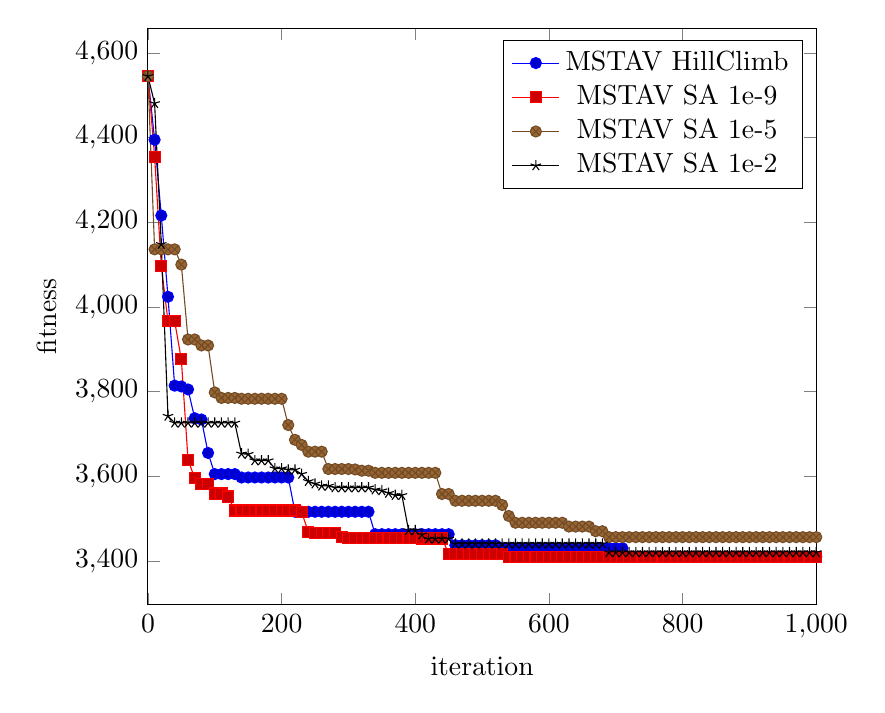
\begin{tikzpicture}
 \begin{axis}[
   width=0.7\textwidth,
   scale only axis,
   xlabel=iteration,
   ylabel=fitness,
   xmin=0,xmax=1000,
   domain=0:1000]
   \addplot coordinates {
     (0,4545)
     (10,4395)
     (20,4216)
     (30,4024)
     (40,3814)
     (50,3812)
     (60,3805)
     (70,3737)
     (80,3734)
     (90,3655)
     (100,3605)
     (110,3605)
     (120,3605)
     (130,3605)
     (140,3597)
     (150,3597)
     (160,3597)
     (170,3597)
     (180,3597)
     (190,3597)
     (200,3597)
     (210,3597)
     (220,3516)
     (230,3516)
     (240,3516)
     (250,3516)
     (260,3516)
     (270,3516)
     (280,3516)
     (290,3516)
     (300,3516)
     (310,3516)
     (320,3516)
     (330,3516)
     (340,3463)
     (350,3463)
     (360,3463)
     (370,3463)
     (380,3463)
     (390,3463)
     (400,3463)
     (410,3463)
     (420,3463)
     (430,3463)
     (440,3463)
     (450,3463)
     (460,3437)
     (470,3437)
     (480,3437)
     (490,3437)
     (500,3437)
     (510,3437)
     (520,3437)
     (530,3430)
     (540,3430)
     (550,3430)
     (560,3430)
     (570,3430)
     (580,3430)
     (590,3430)
     (600,3430)
     (610,3430)
     (620,3430)
     (630,3430)
     (640,3430)
     (650,3430)
     (660,3430)
     (670,3430)
     (680,3430)
     (690,3430)
     (700,3430)
     (710,3430)
     (720,3410)
     (730,3410)
     (740,3410)
     (750,3410)
     (760,3410)
     (770,3410)
     (780,3410)
     (790,3410)
     (800,3410)
     (810,3410)
     (820,3410)
     (830,3410)
     (840,3410)
     (850,3410)
     (860,3410)
     (870,3410)
     (880,3410)
     (890,3410)
     (900,3410)
     (910,3410)
     (920,3410)
     (930,3410)
     (940,3410)
     (950,3410)
     (960,3410)
     (970,3410)
     (980,3410)
     (990,3410)
     (1000,3410)
   };
   \addlegendentry{MSTAV HillClimb}
   \addplot coordinates {
     (0,4545)
     (10,4355)
     (20,4097)
     (30,3966)
     (40,3966)
     (50,3876)
     (60,3639)
     (70,3595)
     (80,3581)
     (90,3581)
     (100,3559)
     (110,3559)
     (120,3552)
     (130,3519)
     (140,3519)
     (150,3519)
     (160,3519)
     (170,3519)
     (180,3519)
     (190,3519)
     (200,3519)
     (210,3519)
     (220,3519)
     (230,3515)
     (240,3468)
     (250,3465)
     (260,3465)
     (270,3465)
     (280,3465)
     (290,3457)
     (300,3454)
     (310,3454)
     (320,3454)
     (330,3454)
     (340,3454)
     (350,3454)
     (360,3454)
     (370,3454)
     (380,3454)
     (390,3454)
     (400,3454)
     (410,3453)
     (420,3453)
     (430,3453)
     (440,3453)
     (450,3417)
     (460,3417)
     (470,3417)
     (480,3417)
     (490,3417)
     (500,3417)
     (510,3417)
     (520,3417)
     (530,3417)
     (540,3410)
     (550,3410)
     (560,3410)
     (570,3410)
     (580,3410)
     (590,3410)
     (600,3410)
     (610,3410)
     (620,3410)
     (630,3410)
     (640,3410)
     (650,3410)
     (660,3410)
     (670,3410)
     (680,3410)
     (690,3410)
     (700,3410)
     (710,3410)
     (720,3410)
     (730,3410)
     (740,3410)
     (750,3410)
     (760,3410)
     (770,3410)
     (780,3410)
     (790,3410)
     (800,3410)
     (810,3410)
     (820,3410)
     (830,3410)
     (840,3410)
     (850,3410)
     (860,3410)
     (870,3410)
     (880,3410)
     (890,3410)
     (900,3410)
     (910,3410)
     (920,3410)
     (930,3410)
     (940,3410)
     (950,3410)
     (960,3410)
     (970,3410)
     (980,3410)
     (990,3410)
     (1000,3410)
   };
   \addlegendentry{MSTAV SA 1e-9}
   \addplot coordinates {
     (0,4545)
     (10,4136)
     (20,4136)
     (30,4136)
     (40,4136)
     (50,4100)
     (60,3923)
     (70,3923)
     (80,3909)
     (90,3909)
     (100,3798)
     (110,3785)
     (120,3785)
     (130,3785)
     (140,3783)
     (150,3783)
     (160,3783)
     (170,3783)
     (180,3783)
     (190,3783)
     (200,3783)
     (210,3721)
     (220,3686)
     (230,3674)
     (240,3658)
     (250,3658)
     (260,3658)
     (270,3617)
     (280,3617)
     (290,3617)
     (300,3617)
     (310,3616)
     (320,3613)
     (330,3613)
     (340,3608)
     (350,3608)
     (360,3608)
     (370,3608)
     (380,3608)
     (390,3608)
     (400,3608)
     (410,3608)
     (420,3608)
     (430,3608)
     (440,3558)
     (450,3558)
     (460,3542)
     (470,3542)
     (480,3542)
     (490,3542)
     (500,3542)
     (510,3542)
     (520,3542)
     (530,3532)
     (540,3506)
     (550,3490)
     (560,3490)
     (570,3490)
     (580,3490)
     (590,3490)
     (600,3490)
     (610,3490)
     (620,3490)
     (630,3481)
     (640,3481)
     (650,3481)
     (660,3481)
     (670,3470)
     (680,3470)
     (690,3456)
     (700,3456)
     (710,3456)
     (720,3456)
     (730,3456)
     (740,3456)
     (750,3456)
     (760,3456)
     (770,3456)
     (780,3456)
     (790,3456)
     (800,3456)
     (810,3456)
     (820,3456)
     (830,3456)
     (840,3456)
     (850,3456)
     (860,3456)
     (870,3456)
     (880,3456)
     (890,3456)
     (900,3456)
     (910,3456)
     (920,3456)
     (930,3456)
     (940,3456)
     (950,3456)
     (960,3456)
     (970,3456)
     (980,3456)
     (990,3456)
     (1000,3456)
   };
   \addlegendentry{MSTAV SA 1e-5}
   \addplot coordinates {
     (0,4545)
     (10,4481)
     (20,4148)
     (30,3742)
     (40,3726)
     (50,3726)
     (60,3726)
     (70,3726)
     (80,3726)
     (90,3726)
     (100,3726)
     (110,3726)
     (120,3726)
     (130,3726)
     (140,3653)
     (150,3652)
     (160,3637)
     (170,3637)
     (180,3637)
     (190,3618)
     (200,3618)
     (210,3615)
     (220,3615)
     (230,3605)
     (240,3588)
     (250,3582)
     (260,3577)
     (270,3577)
     (280,3573)
     (290,3573)
     (300,3573)
     (310,3573)
     (320,3573)
     (330,3573)
     (340,3568)
     (350,3566)
     (360,3560)
     (370,3555)
     (380,3555)
     (390,3472)
     (400,3472)
     (410,3462)
     (420,3452)
     (430,3452)
     (440,3452)
     (450,3452)
     (460,3440)
     (470,3440)
     (480,3440)
     (490,3440)
     (500,3440)
     (510,3440)
     (520,3440)
     (530,3440)
     (540,3440)
     (550,3440)
     (560,3440)
     (570,3440)
     (580,3440)
     (590,3440)
     (600,3440)
     (610,3440)
     (620,3440)
     (630,3440)
     (640,3440)
     (650,3440)
     (660,3440)
     (670,3440)
     (680,3440)
     (690,3420)
     (700,3420)
     (710,3420)
     (720,3420)
     (730,3420)
     (740,3420)
     (750,3420)
     (760,3420)
     (770,3420)
     (780,3420)
     (790,3420)
     (800,3420)
     (810,3420)
     (820,3420)
     (830,3420)
     (840,3420)
     (850,3420)
     (860,3420)
     (870,3420)
     (880,3420)
     (890,3420)
     (900,3420)
     (910,3420)
     (920,3420)
     (930,3420)
     (940,3420)
     (950,3420)
     (960,3420)
     (970,3420)
     (980,3420)
     (990,3420)
     (1000,3420)
   };
   \addlegendentry{MSTAV SA 1e-2}
 \end{axis}
 \end{tikzpicture}
\end{figure}

\end{figure}
\FloatBarrier

\subsection{CBC and MSTAV convergence comparison}
\FloatBarrier

\begin{figure}[hb]
\pgfsetplotmarksize{0pt}
\begin{figure}
 \centering
 \caption{\label{CBCvsMSTAV-d05}CBCvsMSTAV-d05},
 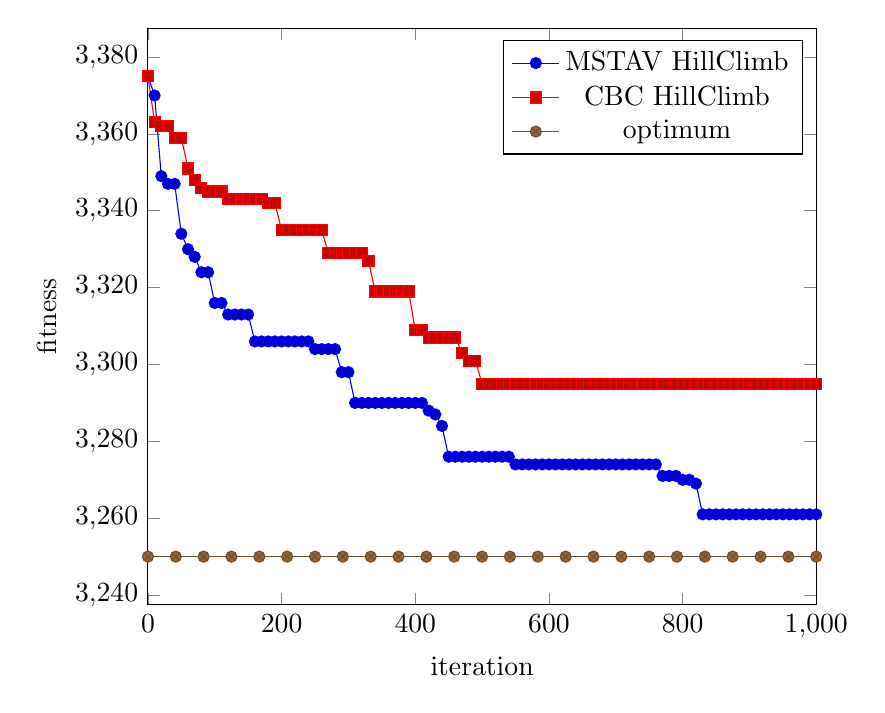
\begin{tikzpicture}
 \begin{axis}[
   width=0.7\textwidth,
   scale only axis,
   xlabel=iteration,
   ylabel=fitness,
   xmin=0,xmax=1000,
   domain=0:1000]
   \addplot coordinates {
     (0,3375)
     (10,3370)
     (20,3349)
     (30,3347)
     (40,3347)
     (50,3334)
     (60,3330)
     (70,3328)
     (80,3324)
     (90,3324)
     (100,3316)
     (110,3316)
     (120,3313)
     (130,3313)
     (140,3313)
     (150,3313)
     (160,3306)
     (170,3306)
     (180,3306)
     (190,3306)
     (200,3306)
     (210,3306)
     (220,3306)
     (230,3306)
     (240,3306)
     (250,3304)
     (260,3304)
     (270,3304)
     (280,3304)
     (290,3298)
     (300,3298)
     (310,3290)
     (320,3290)
     (330,3290)
     (340,3290)
     (350,3290)
     (360,3290)
     (370,3290)
     (380,3290)
     (390,3290)
     (400,3290)
     (410,3290)
     (420,3288)
     (430,3287)
     (440,3284)
     (450,3276)
     (460,3276)
     (470,3276)
     (480,3276)
     (490,3276)
     (500,3276)
     (510,3276)
     (520,3276)
     (530,3276)
     (540,3276)
     (550,3274)
     (560,3274)
     (570,3274)
     (580,3274)
     (590,3274)
     (600,3274)
     (610,3274)
     (620,3274)
     (630,3274)
     (640,3274)
     (650,3274)
     (660,3274)
     (670,3274)
     (680,3274)
     (690,3274)
     (700,3274)
     (710,3274)
     (720,3274)
     (730,3274)
     (740,3274)
     (750,3274)
     (760,3274)
     (770,3271)
     (780,3271)
     (790,3271)
     (800,3270)
     (810,3270)
     (820,3269)
     (830,3261)
     (840,3261)
     (850,3261)
     (860,3261)
     (870,3261)
     (880,3261)
     (890,3261)
     (900,3261)
     (910,3261)
     (920,3261)
     (930,3261)
     (940,3261)
     (950,3261)
     (960,3261)
     (970,3261)
     (980,3261)
     (990,3261)
     (1000,3261)
   };
   \addlegendentry{MSTAV HillClimb}
   \addplot coordinates {
     (0,3375)
     (10,3363)
     (20,3362)
     (30,3362)
     (40,3359)
     (50,3359)
     (60,3351)
     (70,3348)
     (80,3346)
     (90,3345)
     (100,3345)
     (110,3345)
     (120,3343)
     (130,3343)
     (140,3343)
     (150,3343)
     (160,3343)
     (170,3343)
     (180,3342)
     (190,3342)
     (200,3335)
     (210,3335)
     (220,3335)
     (230,3335)
     (240,3335)
     (250,3335)
     (260,3335)
     (270,3329)
     (280,3329)
     (290,3329)
     (300,3329)
     (310,3329)
     (320,3329)
     (330,3327)
     (340,3319)
     (350,3319)
     (360,3319)
     (370,3319)
     (380,3319)
     (390,3319)
     (400,3309)
     (410,3309)
     (420,3307)
     (430,3307)
     (440,3307)
     (450,3307)
     (460,3307)
     (470,3303)
     (480,3301)
     (490,3301)
     (500,3295)
     (510,3295)
     (520,3295)
     (530,3295)
     (540,3295)
     (550,3295)
     (560,3295)
     (570,3295)
     (580,3295)
     (590,3295)
     (600,3295)
     (610,3295)
     (620,3295)
     (630,3295)
     (640,3295)
     (650,3295)
     (660,3295)
     (670,3295)
     (680,3295)
     (690,3295)
     (700,3295)
     (710,3295)
     (720,3295)
     (730,3295)
     (740,3295)
     (750,3295)
     (760,3295)
     (770,3295)
     (780,3295)
     (790,3295)
     (800,3295)
     (810,3295)
     (820,3295)
     (830,3295)
     (840,3295)
     (850,3295)
     (860,3295)
     (870,3295)
     (880,3295)
     (890,3295)
     (900,3295)
     (910,3295)
     (920,3295)
     (930,3295)
     (940,3295)
     (950,3295)
     (960,3295)
     (970,3295)
     (980,3295)
     (990,3295)
     (1000,3295)
   };
   \addlegendentry{CBC HillClimb}
   \addplot {3250.000000};
   \addlegendentry{optimum}
 \end{axis}
 \end{tikzpicture}
\end{figure}

\end{figure}
\FloatBarrier

\subsection{Comparison of found solutions' fitness}
\FloatBarrier
After testing presented algorithms we have made following observations:
\begin{itemize}
\item fitness of solutions found by 2-approximation algorithm is almost always less than 1.1 times optimum,
\item local searches performed well on problem instances with less than thousand of vertices,
\item MSTAV gives better results than CBC most of the time,
\item MSTAV often finds better solutions than 2-approximation algorithm for problem instances with less than thousand of vertices,
\item for graphs with thousands of vertices 2-approximation algorithm finds much better solutions than local seaches.
\end{itemize}

\begin{figure}[hb]
  \centering
  \begin{tabular}[ht]{|l||c|c|c|c|H}
\cline{1-5}
 & 01dEV100K20 & 01sEV1000K150 & 01sEV100K20 & 01dRV100K20 & \\ \cline{1-5}\cline{1-5} 
2-Approximation &3476 & 20605 & 5927 & 24 & \\ \cline{1-5}
MSTAV HillClimb &3376 & 20231 & 5785 & 22 & \\ \cline{1-5}
CBC HillClimb &3654 & 24213 & 6021 & 24 & \\ \cline{1-5}
\end{tabular}
  \caption{Results for sample of SFP tests for graphs with less than thousand vertices}
\end{figure}

\begin{figure}[hb]
  \centering
  \begin{tabular}[ht]{|l||c|c|c|c|c|c|H}
\cline{1-7}
 & alut2764 & b13 & berlin52 & diw0250 & msm3277 & d15 & \\ \cline{1-7}\cline{1-7} 
Optimum &640 & 165 & 1044 & 350 & 869 & 1116 & \\ \cline{1-7}
2-Approximation &710 & 187 & 1078 & 363 & 912 & 1161 & \\ \cline{1-7}
MSTAV HillClimb &662 & 170 & 1044 & 467 & 1089 & 1126 & \\ \cline{1-7}
CBC HillClimb &1044 & 177 & 1103 & 518 & 1222 & 1186 & \\ \cline{1-7}
\end{tabular}
  \caption{Results for sample of STP tests for graphs with less than thousand vertices}
\end{figure}

\begin{figure}[hb]
  \centering
  \begin{tabular}[ht]{|l||c|c|c|c|H}
\cline{1-5}
 & 04sEV1000K250 & 03sEV1000K150 & 01sRV1000K150 & 01sRV1000K250 & \\ \cline{1-5}\cline{1-5} 
2-Approximation &29569 & 17175 & 208 & 262 & \\ \cline{1-5}
MSTAV HillClimb &29624 & 17163 & 196 & 279 & \\ \cline{1-5}
CBC HillClimb &35091 & 21899 & 259 & 365 & \\ \cline{1-5}
\end{tabular}
  \caption{Results for sample of SFP tests for graphs with at least thousand of vertices}
\end{figure}

\begin{figure}[hb]
  \centering
  \begin{tabular}[ht]{|l||c|c|c|c|c|c|H}
\cline{1-7}
 & alue2087 & d11 & diw0445 & e02 & taq0431 & msm3277 & \\ \cline{1-7}\cline{1-7} 
Optimum &1049 & 29 & 1363 & 214 & 897 & 869 & \\ \cline{1-7}
2-Approximation &1122 & 33 & 1453 & 255 & 980 & 912 & \\ \cline{1-7}
MSTAV HillClimb &1375 & 36 & 1827 & 361 & 1484 & 1233 & \\ \cline{1-7}
CBC HillClimb &1698 & 49 & 2321 & 442 & 1519 & 1263 & \\ \cline{1-7}
\end{tabular}
  \caption{Results for sample of STP tests for graphs with at least thousand of vertices}
\end{figure}
\FloatBarrier

\chapter{Metrical Facility Location algorithms}

\section{Problem description}

Problem instance consists of a full bipartite graph $G = (F \cup C, F \times
C)$, where elements of $F$ are called \emph{facilities} and those of $C$ are
called \emph{cities}, $o : F \to \mathbb{R}$ being a cost function of opening
single facility and $c : F \times C \to \mathbb{R}$ being a cost function of
connecting facility with a city. The connection costs satisfy triangle
inequality.

The problem is to find a subset of facilities $O \subset F$ to be opened and an
assignment of cities to opened facilities $a : C \to O$ in such a way that the
total cost $\sum_{f \in O} o(f) + \sum_{c \in C} c(a(c), c)$ is minimized.

\section{Primal-dual schema 3-apx}
We have created efficient implementation of combinatoric approximation
algorithm for the problem as a reference point for other discussed methods. The
algorithm achieves a constant approximation factor of 3 and runs in $\Oh(|F||C|
\log(|F||C|))$ time. It operates in primal-dual fashion trying to find feasible
solution for dual problem with possibly the biggest cost. Detailed description
can be found in TODO. % TODO vasirani

We have introduced a slight modification to original algorithm due to Jain and
Vasirani. Once the set of opened facilities is determined as in original
algorithm we create optimal assignment in $\Oh(|F||C|)$ time by assigning each
city to the closest facility. The assignment presented in original paper is
useful for estimating approximation factor of the algorithm though.

\section{Local Search 3-apx}

Local search with the following properties
guarantees\footnote{\url{http://www.cs.ucla.edu/~awm/papers/lsearch.ps}}
3-apx at local optimum:
\begin{itemize}
\item Search space consists of all subsets of facilities.
\item Fitness function is the same as in problem statement.
\item Valid step is of one of the forms:
	\begin{itemize}
	\item insert one facility to the set
	\item delete one facility from the set
	\item swap one facility from the set with one from outside the set.
	\end{itemize}
\end{itemize}

We have implemented 2 variants of Walkers (see: Local Search Framework design)
for this algorithm:
\begin{itemize}
\item[LS1)] take a random valid step and calculate fitness: $\Oh(|F||C|)$ per iteration
\item[LS2)] find the fittest step among the valid ones: $\Oh(|F|(|F|+|C|))$ per iteration
\end{itemize}

In both cases, time of single iteration is proportional to the problem
instance size. It is therefore necessary to start the local search from
the solution relatively close (in the topology described) to the local
optimum. Intuitively the optimal solution will consist of a small number
of facilities (especially for test cases with uniformly distributed facilities and cities),
therefore the initial solution has been set to an empty set.

\section{Monte Carlo Tree Search}

Because MCTS involves selecting decisions step by step we decided to transform our
standard Facility Location problem into Online Facility Location problem.
The restriction of this approach is that $F = C$, of course one can set
opening costs of some factories to $inf$ to prevent opening one there
but it will be still considered as potential facility to open. \\
Algorithm works as follows, first get the order in which facilities will be
processed, then at each step decide to open or not open facility at given point. \\
Function that estimates fitness of current state is based on
Adam Meyerson's algorithm\footnote{\url{http://www.cs.ucla.edu/~awm/papers/ofl.pdf}},
which is constant competitive for randomized input.

\section{Random Search}

As an additional benchmark for evaluating algorithms' performance, we've implemented
random search, which simply samples solution space at random. Solutions are drawn as follows:
\begin{itemize}
\item draw with uniform distribution the solution size $n \in \{1..|F|\}$.
\item draw $n$ times a facility with uniform distribution.
\item solution is the set of facilities from the previous point.
\end{itemize}

We've empirically shown for the benchmark problem instances, that the near optimal
solutions are small sets. This drawing algorithm is flexible enough to take it
into consideration.

\section{Benchmarks}
To evaluate the algorithms quality we have used UflLib\footnote{\url{http://www.mpi-inf.mpg.de/departments/d1/projects/benchmarks/UflLib/Euklid.html}}
and our "clustered tests". The need for "clustered tests" raised from observation that
uniform distribution is not natural for many real-world situation like city placements
e.g. normally cities are "clustered" around natural resources.

\section{Results}

\begin{figure}[ht]
  \begin{tabular}[ht]{|l||c|c|c|c|c|c|H}
\cline{1-7}
 & 2511EuclS & 1811EuclS & 1211EuclS & 111EuclS & 1911EuclS & 2711EuclS & \\ \cline{1-7}\cline{1-7} 
optimum &99195 & 100189 & 98528 & 96116 & 98617 & 93845 & \\ \cline{1-7}
local search &1.0023 & 1.0165 & 1 & 1.01472 & 1.00671 & 1.00498 & \\ \cline{1-7}
ls fast &1.00605 & 1 & 1 & 1.00744 & 1.01128 & 1 & \\ \cline{1-7}
3 apx &1.19845 & 1.10865 & 1.23954 & 1.09184 & 1.10833 & 1.13838 & \\ \cline{1-7}
random &1.13476 & 1.12494 & 1.12943 & 1.1231 & 1.12784 & 1.11763 & \\ \cline{1-7}
\end{tabular}
\end{figure}


\appendix

\bibliographystyle{plain}
\bibliography{paal}

\end{document}


%%% Local Variables:
%%% mode: latex
%%% TeX-master: t
%%% coding: latin-2
%%% End:
